\documentclass[11pt]{article}
\usepackage[margin=0.85in]{geometry}
\usepackage{amsmath,amssymb,graphicx,booktabs,longtable,array,xcolor,hyperref,fancyhdr,microtype}
\definecolor{ink}{HTML}{164D70}
\hypersetup{colorlinks=true,linkcolor=ink,urlcolor=ink,citecolor=ink}
\setlength{\parindent}{0pt}\setlength{\parskip}{6pt}
\setlength{\headheight}{15pt}
\pagestyle{fancy}\fancyhf{}\fancyhead[L]{\small Computational neurophysiology: frozen suite}
\fancyhead[R]{\small 18 October 2026}\fancyfoot[C]{\thepage}
\setcounter{topnumber}{2}\setcounter{bottomnumber}{2}
\renewcommand{\floatpagefraction}{0.65}
\newcommand{\R}{\mathbb{R}}
\emergencystretch=1em
\begin{document}
\title{Shared priority, distributed memory and task-dependent readout: synthesis of nineteen computational experiments}\author{Visual Attention and Working Memory Project}\date{18 October 2026}\maketitle
\section{The experimental program}
This volume treats the previously trained visual model as one computational subject and applies a common experimental logic to every task. It combines fresh psychophysics, threshold-defined commitment times, spatial-priority perturbations, memory resets, external decoders and population-state analyses. The following nineteen papers contain task-specific hypotheses, methods, results, figures, native condition tables and every-frame representative attention atlases.

The main checkpoint is 204,289, selected under the prior monitoring criterion. The final checkpoint at 220,637 supplies same-movie robustness measurements. Native behavior covers all 437 conditions with 128 trials per condition (55,936 presentations). Additional experiments examine weaker signals, causal manipulations, independent fitting/test populations and explicit VDA counterfactuals. The source data distinguish presentations from unique procedural scenes. Timing manipulations that reuse a scene are clustered together in uncertainty calculations.

\section{Behavior across the entire suite}
\small\begin{longtable}{p{.43\textwidth}rrrr}\toprule Task & Conditions & Trials & Accuracy & AUC\\\midrule\endhead
motion direction & 1 & 128 & 100.0\% & 1.000\\
orientation & 1 & 128 & 100.0\% & 1.000\\
contrast & 1 & 128 & 100.0\% & 1.000\\
spatial frequency & 1 & 128 & 100.0\% & 1.000\\
chromatic increment & 1 & 128 & 100.0\% & 1.000\\
contour & 1 & 128 & 99.2\% & 1.000\\
natural spectrum & 1 & 128 & 100.0\% & 1.000\\
orientation ring & 1 & 128 & 100.0\% & 1.000\\
orientation cued & 4 & 512 & 99.8\% & 1.000\\
motion duration cued & 4 & 512 & 97.5\% & 0.999\\
krauzlis cued motion & 3 & 384 & 95.8\% & 0.995\\
spatial binding & 4 & 512 & 100.0\% & 1.000\\
image recognition & 12 & 1536 & 94.3\% & 0.963\\
vda4 & 3 & 384 & 68.0\% & 0.755\\
vda9 & 3 & 384 & 68.5\% & 0.760\\
vda16 & 3 & 384 & 64.8\% & 0.723\\
memory guided search & 288 & 36864 & 53.1\% & 0.724\\
popout search & 24 & 3072 & 86.4\% & 0.938\\
motion memory search & 81 & 10368 & 97.7\% & 0.999\\
\bottomrule\end{longtable}\normalsize
\begin{figure}[htbp]\centering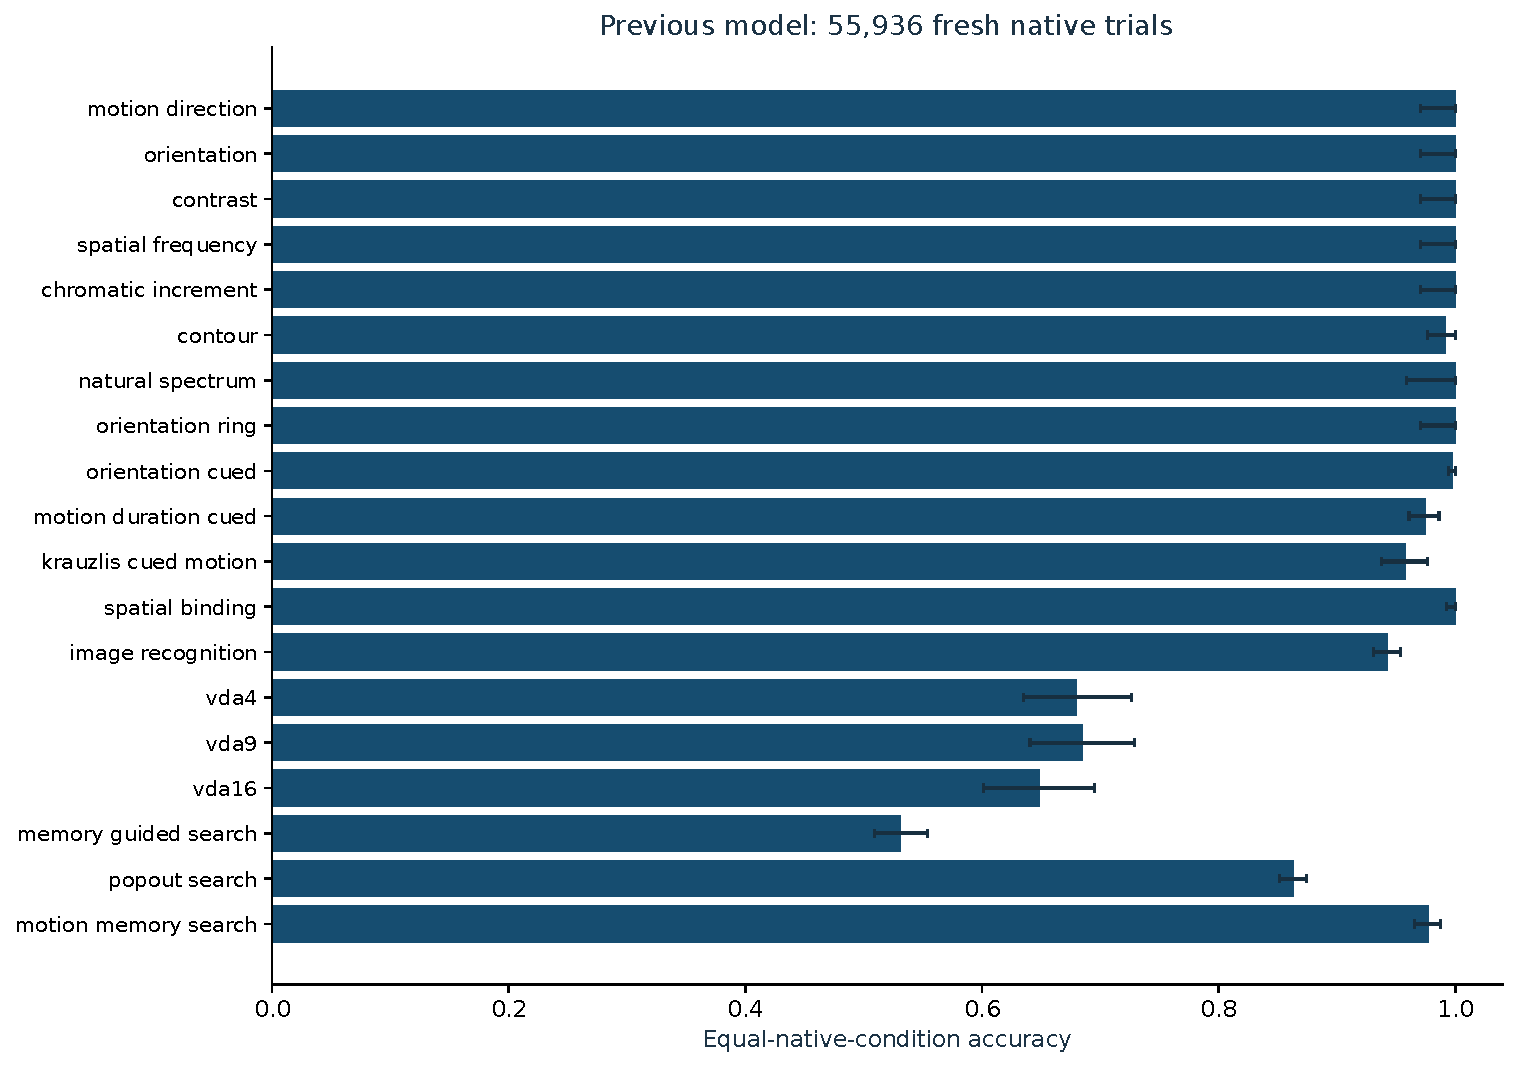
\includegraphics[width=.95\textwidth,height=.7\textheight,keepaspectratio]{suite_behavior.pdf}\caption{Accuracy of the selected previous model on fresh native trials. Each task averages its native conditions equally; the number of conditions differs across tasks. Intervals preserve procedural scene clusters across timing conditions.}\end{figure}
\section{Causal organization}
Across 108 predesignated dose-four evidence comparisons, 41 survived the cross-task Holm correction at 0.05: 5 benefits and 36 costs. This family includes target and alternative-site stimulation and inhibition in each selected condition. The full exploratory dose and epoch sweeps are reported separately in the task papers.

\begin{figure}[htbp]\centering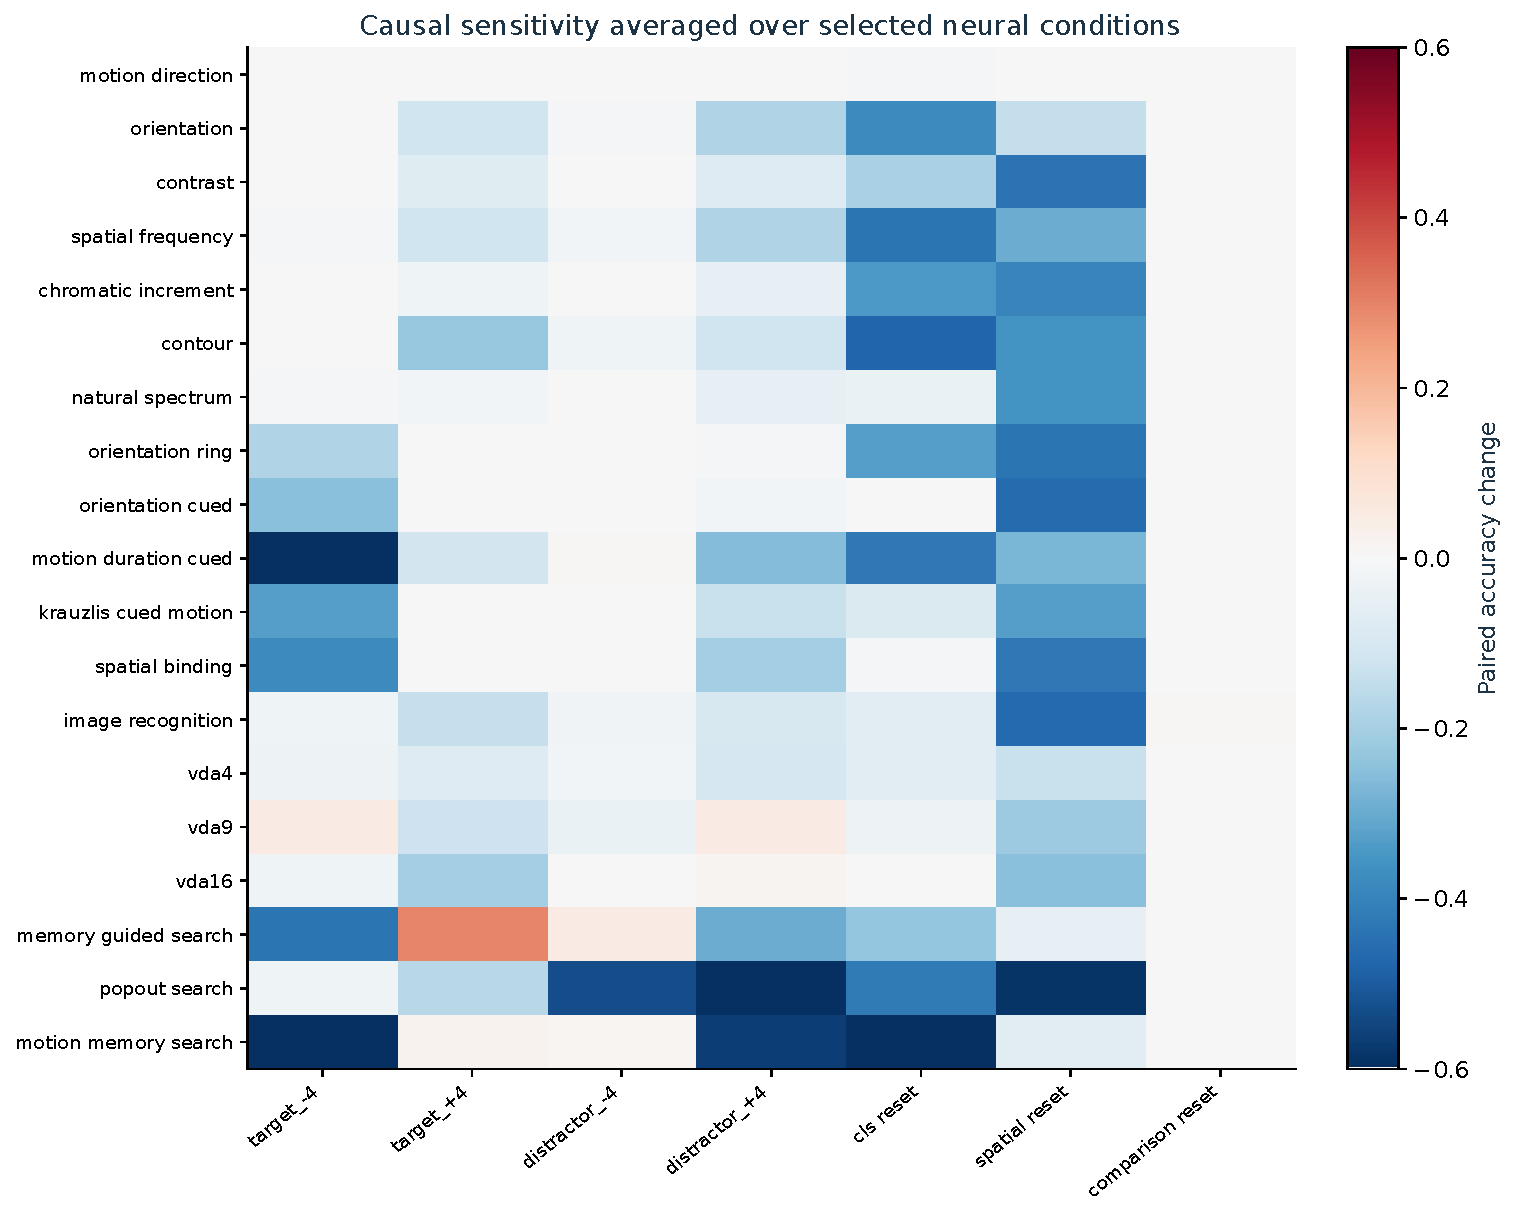
\includegraphics[width=.98\textwidth,height=.74\textheight,keepaspectratio]{suite_causal.pdf}\caption{Causal effects of four spatial interventions and three memory resets. Values average the task-specific selected neural conditions, whose full identities are retained in the protocol. Positive values indicate improved paired accuracy; negative values indicate impairment.}\end{figure}
\subsection{Spatial memory and global memory support distinct tests}
orientation cued: cls: +0.0 percentage points, spatial: -46.1 percentage points, comparison: +0.0 percentage points.

spatial binding: cls: -0.8 percentage points, spatial: -43.0 percentage points, comparison: +0.0 percentage points.

image recognition: cls: -6.2 percentage points, spatial: -46.5 percentage points, comparison: +0.8 percentage points.

memory guided search: cls: -23.3 percentage points, spatial: -5.1 percentage points, comparison: +0.0 percentage points.

motion memory search: cls: -72.7 percentage points, spatial: -6.6 percentage points, comparison: +0.0 percentage points.

These resets measure dependence at a specified instant, followed by normal processing of the remaining movie. A state may contain readable content and still be recoverable from other states after a reset. Conversely, a reset can disrupt subsequent computation even when a restricted linear probe reads the state poorly. Pairing causal and representational results addresses this distinction directly.

\subsection{The VDA counterfactual}
VDA4: catch accuracy change +9.0 points, paired interval [3.1\%, 14.8\%]; cued accuracy change -53.9 points, paired interval [-60.2\%, -48.0\%]; uncued accuracy change +0.8 points, paired interval [-1.2\%, 3.1\%].

VDA9: catch accuracy change +6.6 points, paired interval [1.2\%, 12.5\%]; cued accuracy change -59.0 points, paired interval [-64.8\%, -52.7\%]; uncued accuracy change +3.1 points, paired interval [0.4\%, 5.9\%].

VDA16: catch accuracy change +13.7 points, paired interval [9.4\%, 18.4\%]; cued accuracy change -27.3 points, paired interval [-32.8\%, -21.9\%]; uncued accuracy change -2.7 points, paired interval [-5.9\%, 0.4\%].

These trials pair a certain bottom-right cue with a controlled event at the cue, at top left, or nowhere. The event sequence deliberately tests an expectation violation. All three VDA variants are short enough that the delayed comparison memory is zero; the shared visual-attention and recurrent pathways therefore carry the measured effect. The paired catch condition distinguishes improved detection from increased positive-response tendency.

\subsection{Testing the dual effect away from ceiling}
The exploratory weak-signal follow-up tested 2, 4 and 8 degrees in every VDA size. A joint dual-effect criterion requires both a cued detection cost and an uncued detection benefit under cue inhibition, with both paired tests surviving Holm correction across all 147 follow-up comparisons from the three VDA tasks. This criterion was met in 0 of nine task-strength settings. The complete corrected family is supplied as \texttt{vda\_followup\_family.json}.

\subsection{Holding the array fixed while changing the remembered target}
memory guided search: features\_\allowbreak{}distinct\_\allowbreak{}S8\_\allowbreak{}D12\_\allowbreak{}H8: 99.6\% balanced query accuracy, template probability gain 0.991; features\_\allowbreak{}similar\_\allowbreak{}S8\_\allowbreak{}D12\_\allowbreak{}H8: 86.7\% balanced query accuracy, template probability gain 0.827; fractals\_\allowbreak{}distinct\_\allowbreak{}S8\_\allowbreak{}D12\_\allowbreak{}H8: 45.3\% balanced query accuracy, template probability gain 0.250; fractals\_\allowbreak{}similar\_\allowbreak{}S8\_\allowbreak{}D12\_\allowbreak{}H8: 29.3\% balanced query accuracy, template probability gain 0.049; objects\_\allowbreak{}distinct\_\allowbreak{}S8\_\allowbreak{}D12\_\allowbreak{}H8: 32.4\% balanced query accuracy, template probability gain 0.061; objects\_\allowbreak{}similar\_\allowbreak{}S8\_\allowbreak{}D12\_\allowbreak{}H8: 26.2\% balanced query accuracy, template probability gain 0.013.

motion memory search: motion\_\allowbreak{}A20\_\allowbreak{}S12\_\allowbreak{}D12\_\allowbreak{}H12: 95.3\% balanced query accuracy, template probability gain 0.925; motion\_\allowbreak{}A90\_\allowbreak{}S12\_\allowbreak{}D12\_\allowbreak{}H12: 99.2\% balanced query accuracy, template probability gain 0.987.

The four target queries share identical search pixels within each scene. A query-dependent change therefore reflects the influence of the preceding sample and resulting recurrent state on the same current evidence. The accompanying attention contrast measures whether that influence also changes spatial allocation toward the newly queried location.

\subsection{Usable object information can exceed the learned choice}
Separate linear probes reconstruct the remembered sample from middle-delay spatial memory and the current candidates from local appearance features at the first array frame. An external squared-distance comparison of those reconstructions then chooses a location. Candidate fitting preserves whole scenes in inner validation, and evaluation uses 128 independent scenes per condition. Probe pairs are fitted separately within each family/similarity condition; the original shared agent remains frozen.

\small\begin{longtable}{p{.39\textwidth}rrr}\toprule Family & Agent & Joint readout & Paired Holm p\\\midrule\endhead
features\_\allowbreak{}distinct & 100.0\% & 100.0\% & 1\\
features\_\allowbreak{}similar & 88.3\% & 100.0\% & 0.0001831\\
objects\_\allowbreak{}distinct & 32.0\% & 100.0\% & 7.755e-26\\
objects\_\allowbreak{}similar & 20.3\% & 93.0\% & 2.553e-24\\
fractals\_\allowbreak{}distinct & 46.1\% & 86.7\% & 1.076e-09\\
fractals\_\allowbreak{}similar & 29.7\% & 52.3\% & 0.0002272\\
\bottomrule\end{longtable}\normalsize
The two object conditions show especially large improvements: the available recurrent and visual representations support nearly perfect external matching, while the learned agent makes many errors. This localizes a major component of the failure to how available information is used for comparison and selection. Similar fractals remain more difficult, even though their joint-readout performance also improves. The scientific distinction is between storing information, representing current candidates, and implementing a successful comparison between them.

\section{Neuroscientific interpretation}
Causal attention experiments motivate manipulating a spatial selection signal while measuring perception. Reversible superior-colliculus and frontal-eye-field inactivation can impair cued motion-change performance (Bollimunta, Bogadhi and Krauzlis, 2018). The model permits a corresponding computational question: how does changing priority at a retinotopic location alter the contribution of evidence there and elsewhere? Because the weights form a normalized distribution, this intervention intrinsically redistributes relative influence. The separate location, event and catch measurements make that redistribution behaviorally interpretable.

The memory analyses distinguish content from use. Visual working-memory experiments motivate measuring a sample representation during stimulus absence (Miller, Erickson and Desimone, 1996). Memory-guided search additionally asks how that representation selects a new target among alternatives (Chelazzi and colleagues, 1993). In this architecture, storage can occur across the spatial and global recurrent states, while the query that selects current evidence is computed from the preceding global state. Testing preserved sample information, subsequent target allocation and memory-reset effects therefore provides three complementary observations of the storage-to-selection process.

Population geometry supplies the temporal link. Dynamic prefrontal coding shows why a changing activity pattern can support ongoing computation (Stokes and colleagues, 2013). Temporal generalization asks whether the same fitted linear rule reads information at different times (King and Dehaene, 2014). Here, a shared training-derived projection prevents the axes from changing merely because each time point was analyzed separately. Cross-time readout, state displacement and continuous remembered-feature reconstruction then jointly characterize what persists and how its code evolves.

\section{Using the papers and source data}
Each task paper is self-contained. The HTML index links its PDF, editable LaTeX source, behavioral data, causal data and neural summaries. CSV source tables expose individual native conditions, psychometric points, threshold statistics and intervention effects. Raw trial arrays and metadata remain in the local Results directory. The portable paper archive includes reports, figures, code and summary source data; it excludes model checkpoints and raw stimulus/video datasets.

The analysis is conditional on one trained model. The next replication axis is independently trained models. The fixed threshold procedure supplies computational commitment times, and the intervention definitions specify priority-logit and memory-tensor operations precisely. Those definitions support reproducible comparisons to subsequent architectures without requiring a change in the task suite.

\begin{thebibliography}{99}
\bibitem{sc} Bollimunta A, Bogadhi AR, Krauzlis RJ (2018). Comparing frontal eye field and superior colliculus contributions to covert spatial attention. Nature Communications 9:3553. \url{https://www.nature.com/articles/s41467-018-06042-2}.
\bibitem{wm} Miller EK, Erickson CA, Desimone R (1996). Neural mechanisms of visual working memory in prefrontal cortex of the macaque. Journal of Neuroscience 16:5154-5167. \url{https://pubmed.ncbi.nlm.nih.gov/8756444/}.
\bibitem{it} Chelazzi L, Miller EK, Duncan J, Desimone R (1993). A neural basis for visual search in inferior temporal cortex. Nature 363:345-347. \url{https://pubmed.ncbi.nlm.nih.gov/8497317/}.
\bibitem{stokes} Stokes MG et al. (2013). Dynamic coding for cognitive control in prefrontal cortex. Neuron 78:364-375. \url{https://pubmed.ncbi.nlm.nih.gov/23562541/}.
\bibitem{king} King JR, Dehaene S (2014). Characterizing the dynamics of mental representations: the temporal generalization method. Trends in Cognitive Sciences 18:203-210. \url{https://pmc.ncbi.nlm.nih.gov/articles/PMC5635958/}.
\bibitem{wolfe} Wolfe JM (2021). Guided Search 6.0: An updated model of visual search. Psychonomic Bulletin and Review 28:1060-1092. \url{https://pubmed.ncbi.nlm.nih.gov/33547630/}.
\end{thebibliography}\end{document}